
\section{Autenticare le richieste: la scelta del servizio e la sua integrazione}


Poiché la modalità di autenticazione rappresenta 
un elemento importante per l'esperienza utente, 
in quanto deve assicurare un accesso sicuro all'applicazione mantenendone la semplicità, 
la facilità del processo di autenticazione deve essere garantita.
L'applicazione deve consentire la possibilità di registrarsi creando un nuovo account dedicato,
ma è altrettanto essenziale che permetta agli utenti di farlo anche 
tramite il proprio servizio di autenticazione preferito,
migliorando sicuramente l'usabilità e l'apprezzamento.
Di conseguenza, il sistema di gestione degli accessi deve supportare 
sia la registrazione e la gestione autonoma degli account specifici per il servizio, 
sia fornire l'integrazione con provider di autenticazione esterni.\\
\\
Per lo scopo, Azure fornisce Microsoft Entra ID, 
parte della suite di servizi di autenticazione e autorizzazione Microsoft Entra. 
Sebbene teoricamente in grado di soddisfare i requisiti sopra indicati, 
la complessità della documentazione e le difficoltà riscontrate nell'integrazione con il servizio dell’applicativo
hanno portato a valutare soluzioni alternative negli ambienti cloud.\\
\\
La scelta è quindi ricaduta su Firebase Authentication,
il servizio di autenticazione di Google Cloud Provider, 
che garantisce sia la possibilità di creare account dedicati 
che di collegarsi attraverso altri servizi di autenticazione. 
Presenta librerie di integrazione sia tramite Flutter che tramite C\# 
che risultano facili da utilizzare,
oltre a fornire una piattaforma di gestione con un'interfaccia chiara e intuitiva.
Dal punto di vista economico, il servizio risulta vantaggioso, 
essendo gratuito fino ai cinquantamila utenti mensili attivi.\\
\\
Firebase si integra facilmente con Flutter,
fornendo una libreria che gestisce completamente l'ottenimento e il mantenimento dei token di autenticazione,
a partire dalle credenziali o dalle verifiche precedenti.
Per ogni richiesta che richiede identificazione un servizio apposito intercetta il messaggio, 
recuperando il token e allegandoglielo.
Alla ricezione del messaggio, il server estrae il token dalla richiesta,
per poi contattare Firebase grazie l'astrazione fornita dalla libreria.
Firebase controlla il token e, se corretto,
ne restituisce i dati dell'account relativo.\\
\\
Uno dei requisiti del progetto prevede 
che ogni account sia associato in modo univoco a un singolo utente. 
Durante la fase di registrazione, tuttavia, 
l’account viene inizialmente registrato nel database gestito da Firebase. 
Pertanto, al primo accesso, il server, dopo aver verificato l’autenticità della richiesta, 
provvede a creare una copia dell’account, 
generando poi il relativo nuovo oggetto utente e il primo profilo associato.\\
\\
\begin{figure}[h!]
    \centering
    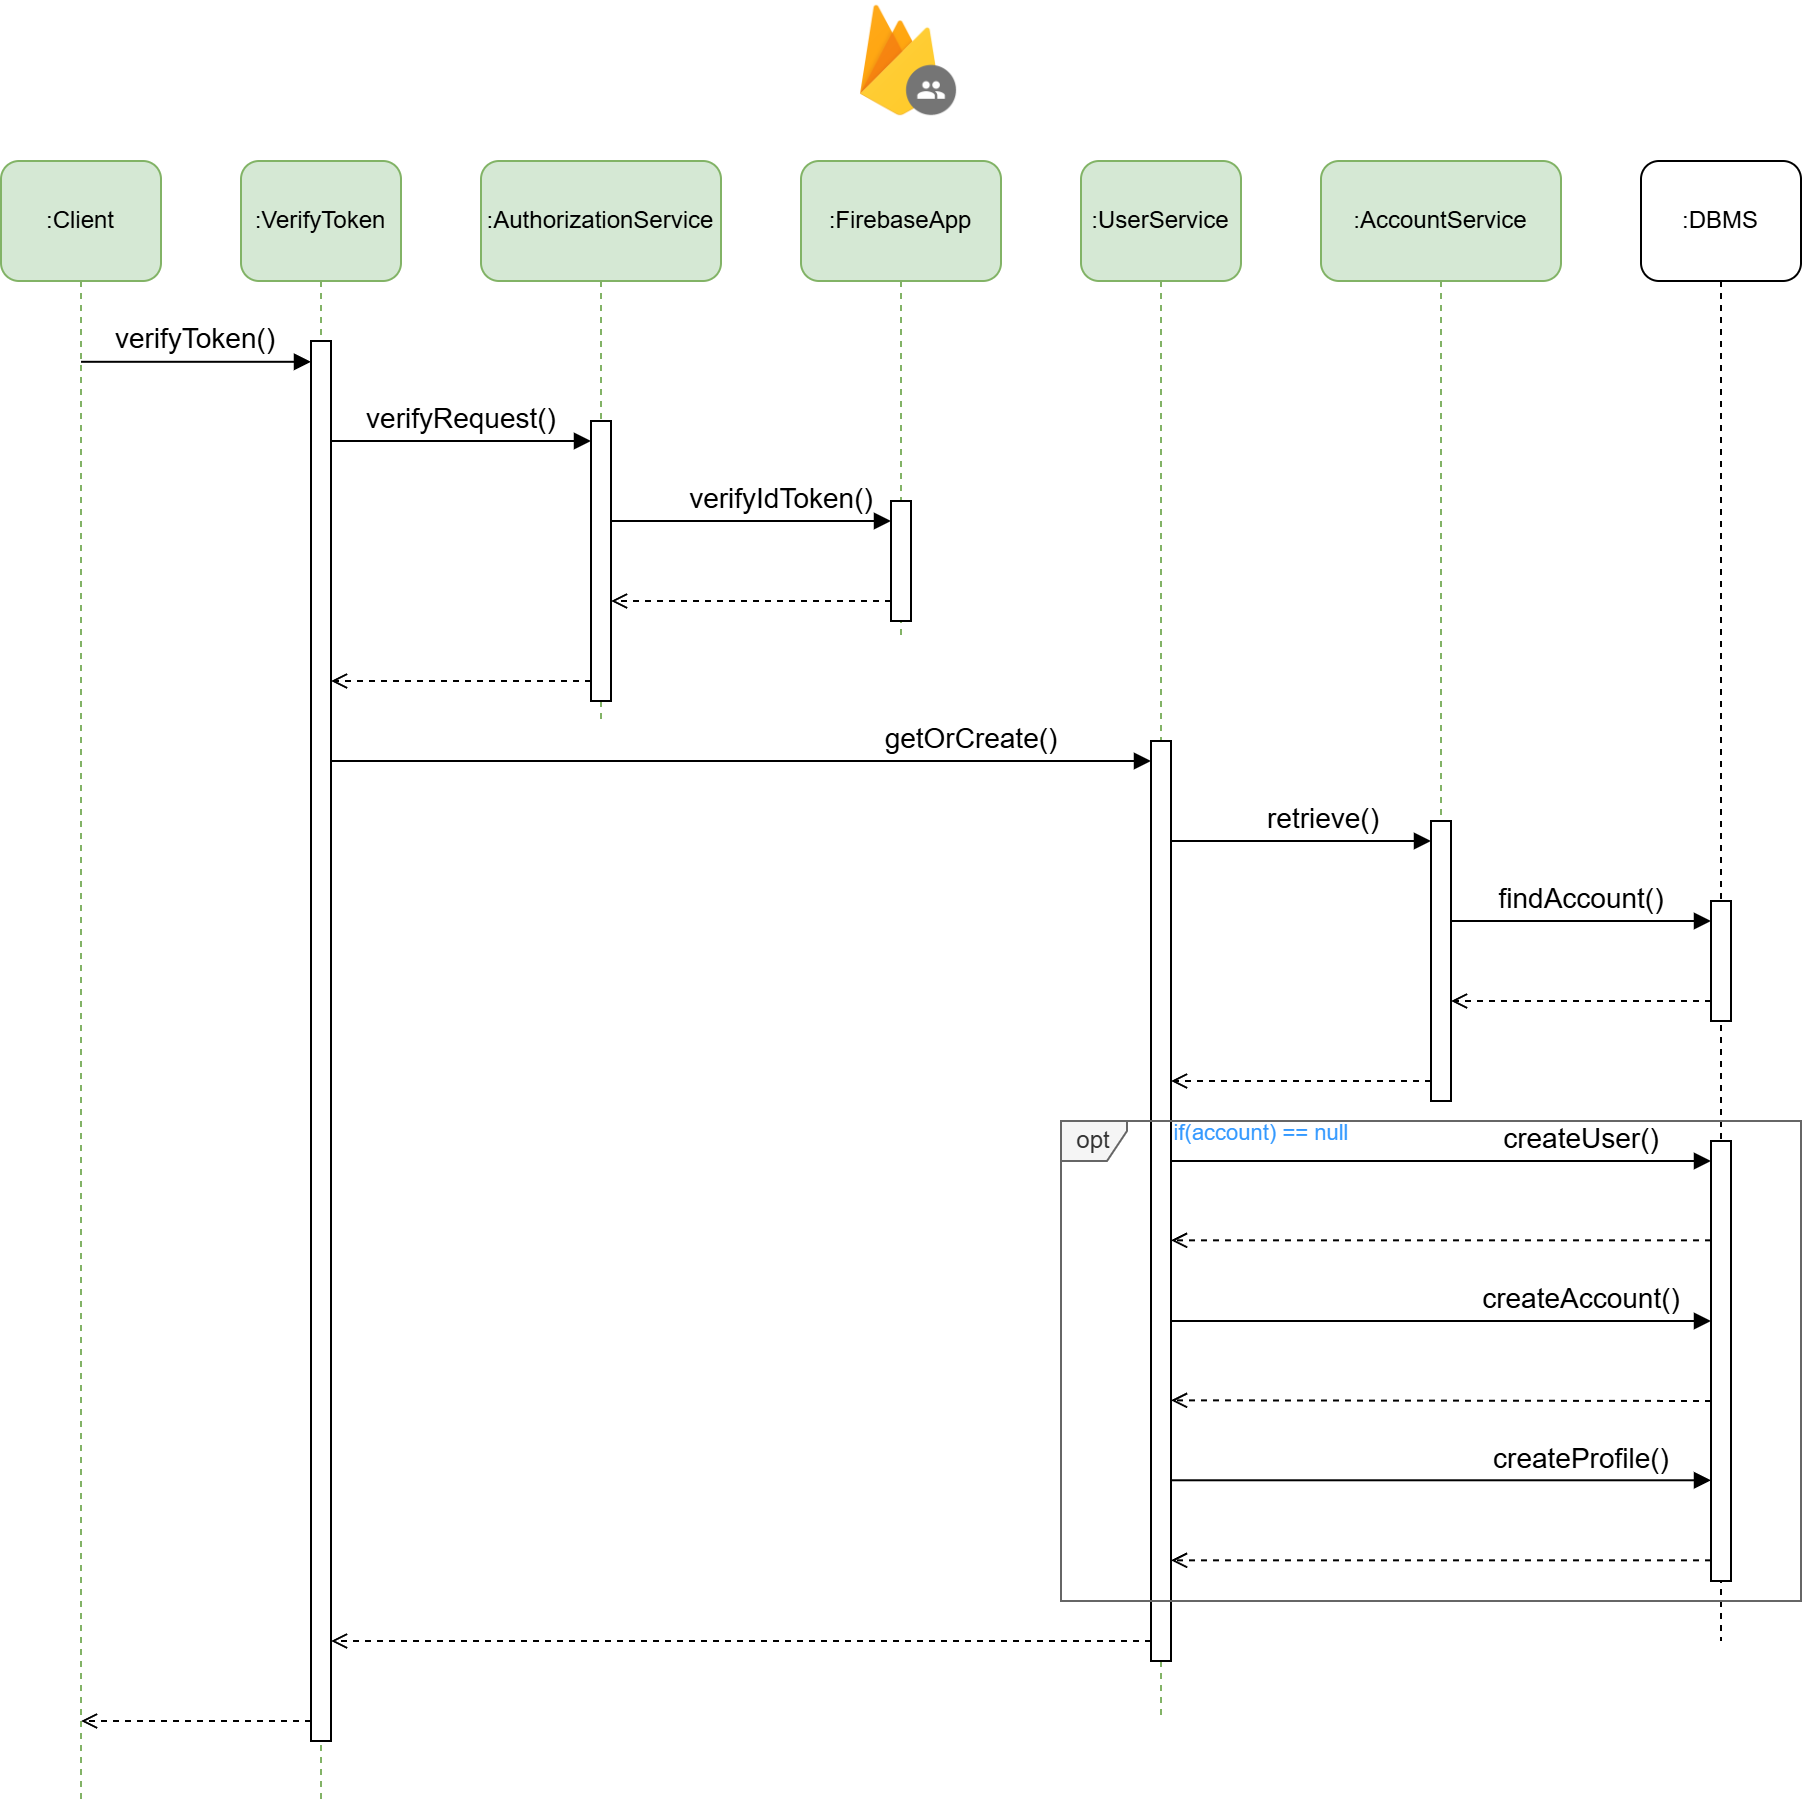
\includegraphics[width=\textwidth]{IIVerifyToken2.png}
    \caption{Diagramma di sequenza per la creazione di un account}
\end{figure}
\clearpage
\section{Uno sguardo sulla sicurezza: segreti e protocolli}

Il collegamento tra i vari componenti all’interno dell’ambiente Azure 
richiede l’utilizzo di chiavi e stringhe di connessione. 
Il salvataggio di tutte le chiavi sensibili è stato affidato al servizio Azure Key Vault,
 un server che permette la centralizzazione dei dati, 
 cifrando il contenuto e garantendo un controllo maggiore sul loro utilizzo. \\
Quando necessario i servizi, in particolare le Azure Functions, 
contatteranno il Key Vault per l'ottenimento delle chiavi necessarie, 
separando di fatto la logica implementativa dai segreti necessari per la sua esecuzione,
riducendo così il rischio di una perdita delle chiavi derivata da un errore dello sviluppo.\\
\\
Le comunicazioni tra i vari componenti devono avvenire in sicurezza, 
garantendo autenticità e confidenzialità. 
Per questo motivo tutte le comunicazioni tra dispositivi client e 
i vari servizi utilizzano la tecnologia TLS, 
che permette di cifrare i messaggi grazie a uno standard collaudato. 
In particolare, le comunicazioni tra i client e Azure Functions, 
così come con Firebase Authentication e il server per la persistenza delle immagini, 
avvengono tramite protocollo HTTPS, 
mentre le comunicazioni con il server per gli aggiornamenti in tempo reale usano il protocollo WSS.\\
\\
Il rischio di saturazione delle risorse viene mitigato 
aggiungendo un duplice controllo sulle dimensioni delle richieste.
In primo luogo si limita la dimensione massima della singola richiesta, 
facendo particolare attenzione alle richieste che contengono immagini, 
controllandola sia nel momento dell'invio che nel momento della ricezione.
Inoltre, alla fine di ogni richiesta più grande di una determinata soglia,
la dimensione viene sommata alle precedenti nell'ultimo periodo e, 
se la somma risulta troppo elevata, viene limitato l'utilizzo per quell'utente.\\
\\
Per evitare un numero eccessivo di richieste totali, 
che possono provocare anch'esse una riduzione del servizio, 
è possibile integrare nel sistema risorse create appositamente da Azure, 
quali Azure DDOS Protection.\\
\\
L’accesso al database è ristretto alle sole risorse Azure, 
garantendo l’isolamento dall’esterno, 
che comprometterebbe altrimenti l’affidabilità dei dati.\\
\\
Infine, l’identificativo di ogni elemento del dominio è nascosto all’utente 
tramite la creazione di codici hash univoci 
che permettono comunque l'identificazione dell'oggetto senza rivelare ulteriori informazioni. 
In particolare, il recupero delle immagini (disponibili in teoria pubblicamente),
avviene grazie a un link univoco dato dalla combinazione degli identificativi dell'evento e dell'immagine. 
Utilizzando i codici di hash diventa molto complicato ritrovare le immagini 
senza essere a conoscenza dei codici, 
che non avendo natura incrementale ma distribuita rende 
indovinare l'unica strategia per trovare un link valido.


\section{Il monitoraggio dei servizi}

Il monitoraggio del sistema è attuato in due modalità: 
tramite il salvataggio dei log e grazie al controllo delle prestazioni del sistema.\\
\\
Relativamente a Firebase Authentication vengono forniti inclusi al servizio 
sia le interfacce per il controllo delle prestazioni che per la gestione dei log. 
Non è quindi richiesta alcuna ulteriore azione.\\
\\
Per monitorare le Azure Functions sarà invece necessario 
affiancargli un'istanza di Azure Application Insights, 
servizio nato appositamente per controllare il funzionamento e la risposta dei servizi Azure. 
Una volta collegato il servizio, infatti, 
Application Insight permette la presentazione e l'analisi di numerose metriche, 
quali il tempo di risposta e il consumo di risorse. 
Consente inoltre di testare la risposta dell'applicativo 
simulando diversi scenari e riassumendo il loro comportamento.\\
\\
La creazione dei log è invece delegata al programmatore, 
in quanto è necessario integrarli nel codice. 
Nel momento della creazione, ogni funzione riceve, tramite dependency injection, 
un servizio Logger che permette la creazione e il salvataggio dei log.
La funzione non dovrà fare altro che chiamare il metodo apposito per generare e salvare un log.
Tali log saranno poi consultabili e analizzabili tramite l’interfaccia fornita da Azure Application Insight.\\
\clearpage